\section{Analysis framework}
\label{sec:analysis_framework}
This work uses the flux, neutrino interaction and detector model described in detail in Ref.~\cite{Abi:2020qib}, implemented in the CAFAna framework~\cite{CAFAna}. This section provides an overview of the key analysis features. Further details on all aspects can be found in Ref.~\cite{Abi:2020qib}.

%% Flux in brief
\subsection{Neutrino flux}
DUNE will operate with two different beam modes, which depend on the polarity of the electromagnetic horns used to focus secondary particles produced after protons from the primary beam line interact in the target. Forward horn current (FHC) corresponds to neutrino-enhanced running, and reverse horn current (RHC) corresponds to antineutrino-enhanced running. In both FHC and RHC there are significant contributions from neutrinos with energies between 0.5--6 GeV, with a flux peak at $\approx$2.5~GeV. The neutrino flux prediction is generated with G4LBNF~\cite{Aliaga:2016oaz,Abi:2020evt}, using the LBNF optimized beam design~\cite{Abi:2020evt}. Flux uncertainties are due to the production rates and kinematic distributions of hadrons produced in the target and the parameters of the beam line, such as horn currents and horn and target positioning (``focusing uncertainties'')~\cite{Abi:2020evt}. They are evaluated using current measurements of hadron production and estimates of alignment tolerances, giving flux uncertainties of approximately 8\% at the first oscillation maximum, which are highly correlated across energy bins and neutrino flavors. A flux covariance as a function of neutrino energy, beam mode, detector, and neutrino species is generated with a ``toy throw'' approach, which is built using variations (``throws'') of the systematics propagated through the full beam line simulation. To reduce the number of parameters used in the fit, the covariance matrix is diagonalized, and each principal component is treated as an uncorrelated nuisance parameter. Only the first $\approx$30 principal components (out of 108) were found to have a significant effect in the analysis and were included. The shapes of the unoscillated fluxes at the ND and FD are similar, and the differences between them are understood at the percent level.

%% Neutrino interactions in brief
\subsection{Neutrino interaction model}
The interaction model used is based on GENIE v2.12.10~\cite{Andreopoulos:2009rq,Andreopoulos:2015wxa}, although the combination of models used is much closer to some of the physics tunes available with GENIE v3.00.06, including a number of uncertainties beyond those provided by either GENIE version. These are motivated by data, although the available (anti)neutrino data taken on argon targets is sparse, leading to an uncertainty model that relies in a number of places on light target (mostly hydrocarbon) data. Variations in the cross sections are implemented either using GENIE reweighting parameters, or with {\em ad hoc} weights of events designed to parameterize uncertainties or cross-section corrections currently not implemented within GENIE. The latter were developed using alternative generators or GENIE configurations, or custom weightings using the NUISANCE package~\cite{Stowell:2016jfr}. Further details about the uncertainties used can be found in Ref.~\cite{Abi:2020qib} (Section 3).

The nuclear model which describes the initial state of nucleons in the nucleus is the Bodek-Ritchie global Fermi gas model~\cite{BodekRitchie}, which includes empirical modifications to the nucleon momentum distribution to account for short-range correlation effects. The quasi-elastic model uses the Llewelyn-Smith formalism~\cite{llewelyn-smith} with a simple dipole axial form factor, and BBBA05 vector form factors~\cite{bbba05}. Nuclear screening effects and uncertainties are included based on the T2K 2017/8 parameterization~\cite{Abe:2018wpn} of the Valencia group's~\cite{nieves1,nieves2} Random Phase Approximation model. The Valencia model of the multi-nucleon, 2p2h, contribution to the cross section~\cite{nieves1,nieves2} is used, as described in Ref.~\cite{Schwehr:2016pvn}. Both MINERvA~\cite{Rodrigues:2015hik} and NOvA~\cite{NOvA:2018gge} have shown that this model underpredicts observed event rates on carbon at relevant neutrino energies for DUNE. Modifications to the model are constructed to produce agreement with MINERvA CC-inclusive data~\cite{Rodrigues:2015hik}, which are used in the analysis to introduce additional uncertainties on the 2p2h contribution, with energy dependent uncertainties, and extra freedom between neutrinos and antineutrinos. Uncertainties are added on scaling the 2p2h prediction from carbon to argon on electron-scattering measurements of short-range correlated (SRC) pairs taken on multiple targets~\cite{Colle:2015ena}, separately for neutrinos and antineutrinos. GENIE uses a modified version of the Rein-Sehgal (R-S) model for pion production~\cite{Rein:1980wg}. A data-driven modification to the GENIE model is included based on reanalyzed neutrino--deuterium bubble chamber data~\cite{Wilkinson:2014yfa,Rodrigues:2016xjj}. The Deep Inelastic Scattering (DIS) model implemented in GENIE uses the Bodek-Yang parametrization~\cite{Bodek:2002ps}, and GRV98 parton distribution functions~\cite{Gluck:1998xa}. Hadronization is described by the AKGY model~\cite{Yang:2009zx}, which uses the KNO scaling model~\cite{Koba:1972ng} for invariant masses $W \leq 2.3$ GeV and PYTHIA6~\cite{Sjostrand:2006za} for invariant masses $W \geq 3$ GeV, with a smooth transition between the two models for intermediate invariant masses. Additional uncertainties developed by the NOvA Collaboration~\cite{nova_2018} to describe their resonance to DIS transition region data are also included. The final state interaction model and uncertainties available in GENIE are retained~\cite{Dytman:2011zz,Dytman:2015taa,intranuke_2009}.

The cross sections include terms proportional to the lepton mass, which are significant at low energies where quasielastic processes dominate. Some of the form factors in these terms have significant uncertainties in the nuclear environment. Separate (and anticorrelated) uncertainties on the cross section ratio $\sigma_\mu/\sigma_e$ for neutrinos and antineutrinos are adopted from Ref.~\cite{Day:2012gb}. Additionally, some $\nu_e$ charged-current (CC) interactions occur at four-momentum transfers where $\nu_\mu$ CC interactions are kinematically forbidden, and so cannot be constrained by $\nu_\mu$ cross-section measurements. To reflect this, a 100\% uncertainty is applied in the phase space present for $\nu_e$ but absent for $\nu_\mu$.

%% ND detector in brief
\subsection{Near detector simulation and reconstruction}
The near detector (ND) hall will be located 574 m downstream of the proton target and $\approx$60~m underground. The reference design for the DUNE ND system is fully described in Ref.~\cite{AbedAbud:2021hpb}, and consists of a liquid argon (LAr) time projection chamber (TPC) referred to as ND-LAr, a magnetized high-pressure gaseous argon TPC (ND-GAr), and an on-axis beam monitor (SAND). Additionally, ND-LAr and ND-GAr are designed to move perpendicular to the beam axis in order to take data at various off-axis angles (the DUNE-PRISM technique). ND-LAr is a modular detector based on the ArgonCube design~\cite{argoncube_loi, Dwyer:2018phu, arclight}, with a total active LAr volume of $105$~m$^{3}$ (a LAr mass of 147 tons). ND-GAr is implemented in this analysis as a cylindrical TPC filled with a 90/10 mixture of argon and CH$_{4}$ at 10 bar, surrounded by a granular, high-performance electromagnetic calorimeter (ECal). ND-GAr sits immediately downstream of the LAr cryostat and serves as a muon spectrometer for ND-LAr~\cite{AbedAbud:2021hpb}.

Neutrino interactions are simulated in the active volume of ND-LAr. The propagation of neutrino interaction products through the ND-LAr and ND-GAr detector volumes is simulated using a Geant4-based program~\cite{Agostinelli:2002hh}. As pattern recognition and reconstruction software has not yet been fully developed for the ND, this analysis uses a parameterized reconstruction based on the Geant4 simulated energy deposits in active detector volumes.

Only CC-inclusive interactions originating in the LAr are considered in this analysis, with a fiducial volume (FV) which excludes 50 cm from the sides and upstream edge, and 150 cm from the downstream edge of the active region, containing a total fiducial mass of $\approx$50~t. Most muons with kinetic energies greater than 1 GeV exit ND-LAr. Energetic forward-going muons pass into ND-GAr, where their momentum and charge are reconstructed by curvature. Muon energy is reconstructed by range for tracks that stop in the LAr, and the charge cannot be determined event-by-event. Events with muons that exit the LAr active volume and do not match to a track in ND-GAr are rejected, as the muon momentum is not well reconstructed. For FHC beam running, the wrong-sign background is small and the charge is assumed to be negative for all LAr-contained muons. For RHC beam running, a Michel electron is required at the end of these stopped tracks to suppress the wrong-sign $\mu^-$ by a factor of four.

All generated muons and charged pions are evaluated as potential muon candidates. Tracks are classified as muons if their length is at least 1 m, and their mean energy deposit is less than 3 MeV/cm. The minimum length requirement imposes an effective threshold on the true muon kinetic energy of about 200 MeV, but greatly suppresses potential neutral current (NC) backgrounds with low-energy, non-interacting charged pions. Charged-current events are required to have exactly one muon candidate, and if the charge is reconstructed by curvature, it must be of the appropriate sign. Hadronic energy in the ND is reconstructed by summing all charge deposits in the LAr active volume that are not associated with the muon. To remove events where the hadronic energy is badly reconstructed due to charged particles exiting the detector, a veto region is defined as the outer 30 cm of the active volume on all sides, and events with more than 30 MeV total energy deposited in the veto region are rejected. Only a fraction of neutron kinetic energy is typically observed (24\% on average with large fluctuations), resulting in poor energy reconstruction of events with energetic neutrons. The reconstructed neutrino energy, $E_{\nu}^{\mathrm{rec}} = E_{\mu}^{\mathrm{rec}} + E_{\mathrm{had}}^{\mathrm{rec}}$, is the sum of the reconstructed hadronic energy, $E_{\mathrm{had}}^{\mathrm{rec}}$, and the reconstructed muon energy, $E_{\mu}^{\mathrm{rec}}$. The reconstructed inelasticity, $y_{\mathrm{rec}} = 1 - E_{\mu}^{\mathrm{rec}}/E_{\nu}^{\mathrm{rec}}$, is the fraction of the neutrino energy that is carried by hadrons.

%% FD description
\subsection{Far detector simulation and reconstruction}
\label{sec:fd}
The DUNE FD design consists of four separate LArTPC detector modules, each with a total LAr mass of 17 kt, installed $\approx$1.5~km underground at the Sanford Underground Research Facility (SURF)~\cite{Abi:2018dnh}. The technologies to be deployed for the four modules and their order of construction are still under investigation, so in this analysis, only the single-phase design with a horizontal drift~\cite{Abi:2020loh} is used. In this design, signals from drift electrons in the 13.3 $\times$ 12.0 $\times$ 57.5 m$^{3}$ active volume are read out by $\approx$5~mm spaced wires in anode readout planes. Scintillation light produced at the time of the neutrino interaction is detected and used to reconstruct the start time of the electron drift. We have developed a full simulation chain, which generates neutrino events in a Geant4 model of the FD geometry and simulates the electronics readout. We have developed a reconstruction package to calculate efficiencies and reconstructed neutrino energy estimators for the four CC-inclusive FD samples used in the analysis (\numu-like FHC, \nue-like FHC, \anumu-like RHC and \anue-like RHC).

The electronics response to the ionization electrons and scintillation light is simulated in the wire planes and photon detectors, respectively. Algorithms are applied to remove the impact of the LArTPC electric field and electronics response from the raw detector signal to identify hits, and to cluster hits that may be grouped together due to proximity in time and space. Clusters from different wire planes are matched to form high-level objects such as tracks and showers using the Pandora toolkit~\cite{Marshall:2015rfa,Acciarri:2017hat}. Event classification is carried out through image recognition techniques using a convolutional neural network~\cite{cvn_paper} which classifies events as $\nu^{\bracketbar}_{\mu}$-CC, $\nu^{\bracketbar}_{e}$-CC, $\nu^{\bracketbar}_{\tau}$-CC, and NC. The $\nue^{\bracketbar}$ and $\numu^{\bracketbar}$ efficiencies in both beam modes exceed 90\% in the flux peak.

The neutrino energy for $\,\nu^{\bracketbar}_{\mu}$-CC ($\,\nu^{\bracketbar}_{e}$-CC) events is estimated by the sum of the energy of the longest reconstructed track (highest energy reconstructed electromagnetic shower) and the hadronic energy. For both event types, the hadronic energy is estimated from the charge of reconstructed hits that are not in the primary track or shower, and corrections are applied to each hit charge for recombination and electron lifetime effects. For $\nu^{\bracketbar}_{\mu}$-CC events, the energy of the longest track is estimated by range if the track is contained or by multiple Coulomb scattering if it is exiting. For 0.5--4 GeV neutrino energies, the observed neutrino energy resolution is 15--20\%. The muon energy resolution is 4\% for contained tracks and 18\% for exiting tracks. The electron energy resolution is approximately $4\% \oplus 9\%/\sqrt{E}$. The hadronic energy resolution is 34\%.

%% Detector systematics
\subsection{Detector systematics}
Detector effects impact the event selection efficiency as well as the reconstruction of neutrino energy and inelasticity (the variables used in the oscillation fits). The main sources of detector systematic uncertainties are limitations of the expected calibration and modeling of particles in the detector. Important differences between the ND and FD LArTPC design, size, detector environment, and calibration strategy, lead to uncertainties that do not fully correlate between the two detectors. The degree of correlation is under active study, but in this analysis they are treated as being completely uncorrelated. Detailed simulations of detector effects are under development. In this analysis, uncertainties on the energy scale, energy resolution, particle responses, and detector acceptance are included to encapsulate these effects. The absolute scale uncertainties shift the reconstructed energy distributions, while the resolution uncertainties narrow or broaden them.

An uncertainty on the overall energy scale is included in the analysis presented here, as well as particle energy scale and resolution uncertainties that are separate and uncorrelated between four particle classes: muons, charged hadrons, neutrons, and electromagnetic showers. In the ND, muons reconstructed by range in LAr and by curvature in the ND-GAr are treated separately and assigned uncorrelated uncertainties. For each class of particle, uncertainties on the energy scale are introduced as a function of the reconstructed particle energy, $E$, with a constant term, a term proportional to $\sqrt{E}$, and a term proportional to $1/\sqrt{E}$. A 10\% uncertainty on the energy resolution is also included, and treated as uncorrelated between the four particle classes. The parameters produce a shift to the kinematic variables in an event, as opposed to simply assigning a weight to each simulated event. The scale of the uncertainties is motivated by what has been achieved in recent experiments, including calorimetric based approaches (NOvA, MINERvA) and LArTPCs (LArIAT, MicroBooNE, ArgoNeut).

In addition to impacting energy reconstruction, the E-field model also affects the definition of the FD FV, which is sensitive to electron drift. An additional 1\% uncertainty is therefore included on the total fiducial mass, which is conservatively treated as uncorrelated between the $\nu^{\bracketbar}_{\mu}$ and $\nu^{\bracketbar}_{e}$ samples due to the potential distortion caused by large electromagnetic showers in the electron sample.

The FD is sufficiently large that acceptance is not expected to vary significantly as a function of event kinematics. However, the ND acceptance does vary as a function of both muon and hadronic kinematics due to various containment criteria. Uncertainties are evaluated on the muon and hadron acceptance at the ND based on the change in the acceptance as a function of muon kinematics and true hadronic energy.

%% Sensitivity method
\subsection{Sensitivity Methods}
Systematics are implemented in the analysis using one-dimensional response functions for each analysis bin, and oscillation weights are calculated exactly, in fine (50 MeV) bins of true neutrino energy. For a given set of inputs --- flux, oscillation parameters, cross sections, detector energy response matrices, and detector efficiency --- an expected event rate can be produced. Minimization is performed using the {\sc minuit}~\cite{James:1994vla} package.

\begin{table}[htbp]
    \centering
    \begin{tabular}{lcc}
      \hline
      Parameter &    Central value & Relative uncertainty \\
      \hline\hline
      $\theta_{12}$ & 0.5903 & 2.3\% \\ 
      $\theta_{23}$ (NO) & 0.866  & 4.1\% \\ 
      $\theta_{23}$ (IO) & 0.869  & 4.0\% \\
      $\theta_{13}$ (NO) & 0.150  & 1.5\% \\ 
      $\theta_{13}$ (IO) & 0.151  & 1.5\% \\
      $\Delta m^2_{21}$ & 7.39$\times10^{-5}$~eV$^2$ & 2.8\% \\
      $\Delta m^2_{32}$ (NO) & 2.451$\times10^{-3}$~eV$^2$ &  1.3\% \\
      $\Delta m^2_{32}$ (IO) & -2.512$\times10^{-3}$~eV$^2$ &  1.3\% \\
      $\rho$ & 2.848 g cm$^{-3}$ & 2\% \\
      \deltacp (NO) & -2.53 (rad.) & -- \\
      \deltacp (IO) & -1.33 (rad.) & -- \\
      \hline
    \end{tabular}
    \caption{Central value and relative uncertainty of neutrino oscillation parameters from a global fit~\cite{Esteban:2018azc,nufitweb} to neutrino oscillation data. The matter density is taken from Ref.~\cite{Roe:2017zdw}. Because the probability distributions are somewhat non-Gaussian (particularly for $\theta_{23}$), the relative uncertainty is computed using 1/6 of the 3$\sigma$ allowed range from the fit, rather than 1/2 of the 1$\sigma$ range. For $\theta_{23}$, $\theta_{13}$, and $\Delta m^2_{31}$, the best-fit values and uncertainties depend on whether NO or IO is assumed. The best fit for \deltacp is used as a test point in the analysis, but no uncertainty is assigned.}
    \label{tab:oscpar_nufit}
\end{table}

Oscillation sensitivities are obtained by simultaneously fitting the \numu-like FHC, \nue-like FHC, \anumu-like RHC and \anue-like RHC FD spectra along with the $\nu_{\mu}$ FHC and $\bar{\nu}_{\mu}$ RHC samples from the ND. In the studies, all oscillation parameters shown in Table~\ref{tab:oscpar_nufit} are allowed to vary. Gaussian penalty terms (taken from Table~\ref{tab:oscpar_nufit}) are applied to $\theta_{12}$, \dm{21}, and the matter density, $\rho$, of the Earth along the DUNE baseline~\cite{Roe:2017zdw}. Some studies presented in this work include a Gaussian penalty term on $\theta_{13}$ (also taken from NuFIT 4.0, given in Table~\ref{tab:oscpar_nufit}), which is precisely measured by experiments sensitive to reactor antineutrino disappearance~\cite{Abrahao:2020ztg,Adey:2018zwh,Bak:2018ydk}. The remaining parameters, \sinst{23}, $\Delta m^{2}_{32}$, and \deltacp are allowed to vary freely, with no penalty terms. The penalty terms are treated as uncorrelated with each other, and uncorrelated with other parameters.

Flux, cross-section, and FD detector parameters are allowed to vary in the fit, but are constrained by a penalty term corresponding to the prior uncertainty. ND detector uncertainties are included via a covariance matrix based on the shape difference between ND prediction and the ``data'' (which comes from the simulation in this sensitivity study). The covariance matrix is constructed with a throwing technique. For each ``throw'', all ND energy scale, resolution, and acceptance parameters are simultaneously thrown according to their respective uncertainties, and the modified prediction is produced by varying the relevant quantities away from the nominal prediction according to the thrown parameter values. The bin-to-bin covariance is determined by comparing the resulting spectra with the nominal prediction, in the same binning as is used in the oscillation sensitivity analysis.

The compatibility of a particular oscillation hypothesis with both ND and FD data is evaluated using the standard Poisson log-likelihood ratio~\cite{Tanabashi:2018oca}:
\begin{linenomath*}
  \begin{equation}
    \begin{aligned}
      \chi^2(\vec{\vartheta}, \vec{x}) &= -2\log\mathcal{L}(\vec{\vartheta}, \vec{x}) \\
      &= 2\sum_i^{N_{\rm bins}}\left[ M_i(\vec{\vartheta}, \vec{x})-D_i+D_i\ln\left({D_i\over M_i(\vec{\vartheta}, \vec{x})}\right) \right] \\
      &+ \sum_{j}^{N_{\mathrm{systs}}}\left[ \frac{\Delta x_{j}}{\sigma_{j}} \right]^{2} \\
      &+ \sum^{N^{\mathrm{ND}}_{\mathrm{bins}}}_{k}\sum^{N^{\mathrm{ND}}_{\mathrm{bins}}}_{l} \left(M_k(\vec{x})-D_k \right) V^{-1}_{kl}\left(M_l(\vec{x})-D_l \right),
    \end{aligned}
    \label{eq:chisq}
  \end{equation}
\end{linenomath*}
where $\vec{\vartheta}$ and $\vec{x}$ are the vector of oscillation parameter and nuisance parameter values, respectively; $N_{\rm bins}$ is the total number of ND and FD bins used in the analysis; $N^{\mathrm{ND}}_{\mathrm{bins}}$ is the number of ND bins; $M_i(\vec{\vartheta}, \vec{x})$ and $D_{i}$ are the MC expectation and fake data in the $i$th reconstructed bin (summed over all selected samples), with the oscillation parameters neglected for the ND; $\Delta x_{j}$ and $\sigma_{j}$ are the difference between the nominal and current value, and the prior uncertainty on the $j$th nuisance parameter; and $V_{kl}$ is the covariance matrix between ND bins described previously. To protect against false minima, all fits are repeated starting at four different \deltacp values (-$\pi$, -$\pi$/2, 0, $\pi$/2), in both mass orderings, and in both \sinst{23} octants, and the lowest obtained $\chi^{2}$ value is taken as the true minimum.

\begin{table}
  \centering
  \begin{tabular}{lcc}
    \hline
    Parameter & Prior & Range\\ \hline\hline
    $\sin^{2}\theta_{23}$ & Uniform & [0.4; 0.6] \\
    $|\Delta m^{2}_{32}|$ ($\times 10^{-3}$ eV$^{2}$) & Uniform & $|[2.3;2.7]|$ \\
    \deltacp ($\pi$) & Uniform & [-1;1] \\
    $\theta_{13}$ (NO) & Gaussian & 0.1503 $\pm$ 0.0023 (rad.)  \\
    $\theta_{13}$ (IO) & Gaussian & 0.1510 $\pm$ 0.0023 (rad.)  \\
    \hline
  \end{tabular}
  \caption{Treatment of the oscillation parameters for the simulated data set studies. The value and uncertainty for $\theta_{13}$ in both NO and IO used in the analysis come from NuFIT 4.0~\cite{Esteban:2018azc,nufitweb}.}
  \label{table:OA_throw}
\end{table}
Two approaches are used for the sensitivity studies presented in this work. Asimov studies~\cite{Cowan:2010js} are carried out (in Section~\ref{sec:run_plan_opt}) in which the fake (Asimov) dataset is the same as the nominal MC. In these, the true value of all systematic uncertainties and oscillation parameters are set to their nominal value (see Table~\ref{tab:oscpar_nufit}) except the parameters of interest, which are set to a test point. Then a fit is carried out in which all parameters can vary, constrained by their prior uncertainty where applicable. For the smallest exposures investigated with an Asimov study in this work, all samples have at least 100 events, satisfying the Gaussian approximation inherent in the Asimov method. Toy throw studies are performed (in Sections~\ref{sec:cp_sens} and~\ref{sec:mh_sens}) in which an ensemble of systematic, oscillation parameter and statistical throws are made. Systematic throws are made according to their prior Gaussian uncertainties, oscillation parameters are randomly chosen as described in Table~\ref{table:OA_throw}, and Poisson fluctuations are then applied to all analysis bins, based on the mean event count for each bin after the systematic adjustments have been applied. For each throw in the ensemble, the test statistic is minimized, and the best-fit value of all parameters is determined. The expected resolution for parameters of interest are then determined from the spread in the distribution of their post-fit values.

Asimov studies are computationally efficient, and for Gaussian parameters and uncertainties, give a good sense of the median sensitivity of an experiment. Toy throwing studies are computationally expensive, fully explore the parameter space, and make fewer assumptions about the behavior of parameters and uncertainties.


\subsection{Near and far detector samples and statistics}
In this work, the sensitivity as a function of FD exposure is explored and results are reported in terms of kt-MW-yr, which does not assume any specific FD or beam intensity staging scenario. However, the ND used in this analysis (ND-LAr with a dowstream muon spectrometer) is assumed not to be staged, and as such the ND sample size corresponding to a particular FD exposure will vary based on the staging scenario. The nominal staging scenario from Ref.~\cite{Abi:2020qib} is therefore retained for the purpose of normalizing the ND samples at each FD exposure. In that scenario, a 7 year exposure corresponds to 336 kt-MW-yr at the FD, and 480 t-MW-yr at the ND, summed over both beam modes. The ND statistics used in this analysis are scaled assuming this ratio throughout, using the same fraction of exposure in each beam mode as used at the FD. The ND samples used in this analysis are relatively quickly systematics limited in both beam modes, and so these approximations are unlikely to have a significant impact on the results.

\begin{figure*}
  \centering
  \subfloat[FHC]{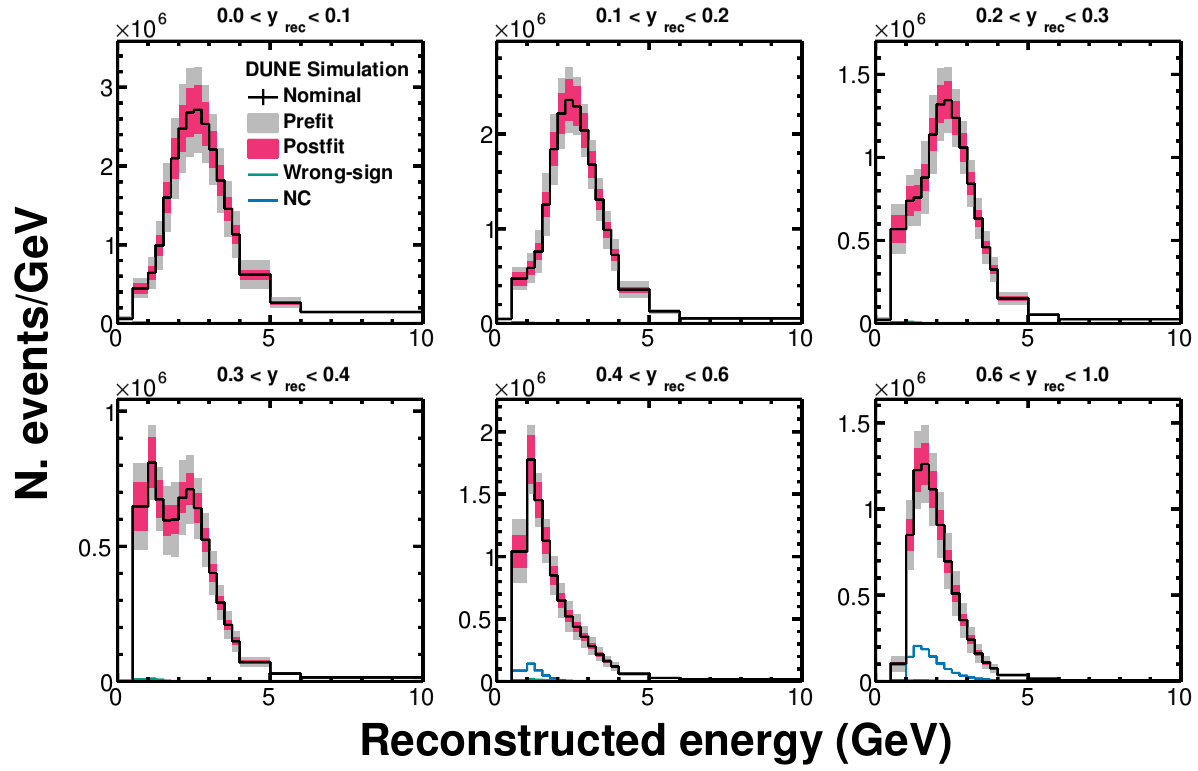
\includegraphics[width=0.8\linewidth]{ND_FHC_ndfd100ktMWyr_allsyst_asimov0_th13_constraint.png}}\\
  \subfloat[RHC]{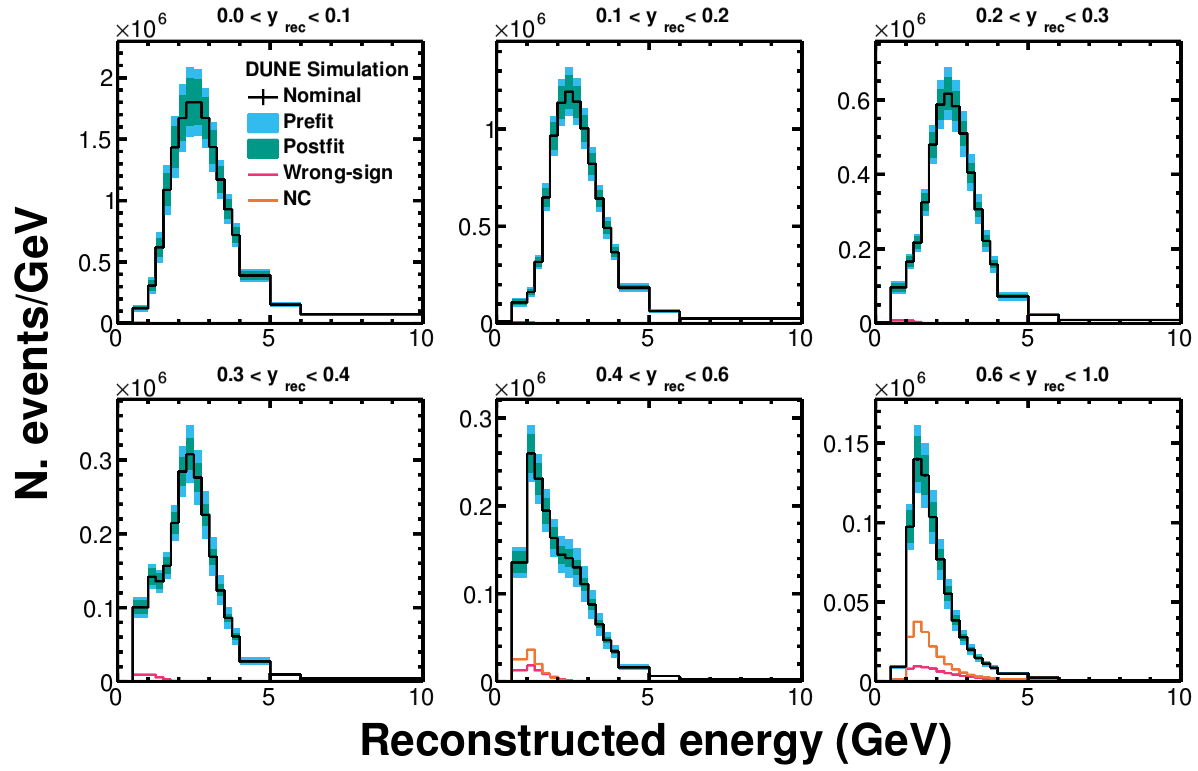
\includegraphics[width=0.8\linewidth]{ND_RHC_ndfd100ktMWyr_allsyst_asimov0_th13_constraint.png}}
  \caption{ND samples in both FHC and RHC, shown in the reconstructed neutrino energy and reconstructed inelasticity binning ($y_{\mathrm{rec}}$) used in the analysis, for a 105 t-MW-yr exposure (equivalent to a 100 kt-MW-yr exposure at the FD), with an equal split between FHC and RHC. The size of the systematic uncertainty bands from all of the flux, cross-section and ND detector systematics used in the analysis are shown, as well as the postfit uncertainty bands obtained by performing an Asimov fit to the ND data. NC backgrounds and wrong-sign contributions to the total event rate are also shown. Statistical uncertainties are too small to be visible on this plot scale.}
 \label{fig:nd_samples}
\end{figure*}
The oscillation analysis presented here includes two CC-inclusive samples originating in the ND-LAr FV, an FHC $\nu_{\mu}$ and an RHC $\bar{\nu}_{\mu}$ sample. These samples are both binned in two dimensions, as a function of reconstructed neutrino energy and inelasticity, $y_{\mathrm{rec}} = 1 - E^{\mathrm{rec}}_{\mu}/E^{\mathrm{rec}}_{\nu}$. The sample distributions for both FHC and RHC are shown in Figure~\ref{fig:nd_samples} for an exposure of 105 t-MW-yr, corresponding to 100 kt-MW-yr at the far detector with the assumptions stated above. The size of the systematic uncertainty bands from all of the flux, cross-section and ND detector systematics used in the analysis and described above are shown, as well as the postfit uncertainty bands obtained by performing an Asimov fit to the ND data. It is clear that even after a relatively small exposure of 105 t-MW-yr, the ND samples are very high statistics, and are systematics limited in the binning used in the analysis. Backgrounds in the $\nu^{\bracketbar}_{\mu}$-CC samples are also shown in Figure~\ref{fig:nd_samples}. NC backgrounds are predominantly from NC $\pi^{\pm}$ production where the pion leaves a long track and does not shower. Wrong-sign contamination in the beam is a background where the charge of the muon is not reconstructed, which particularly affects low reconstructed neutrino energies in RHC. The wrong-sign background is also larger at high reconstructed inelasticity, $y_{\mathrm{rec}}$, due to the kinematics of neutrino and antineutrino scattering.

\begin{figure}[htbp]
 \subfloat[FHC]{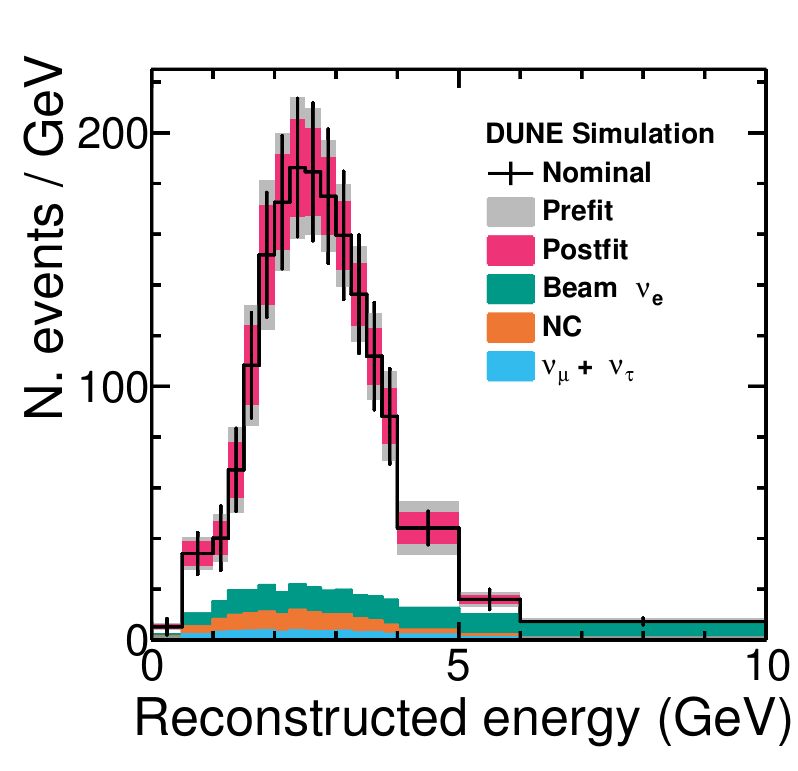
\includegraphics[width=0.8\linewidth]{FD_nue_FHC_ndfd100ktMWyr_allsyst_asimov0_th13_constraint.png}}\\
 \subfloat[RHC]{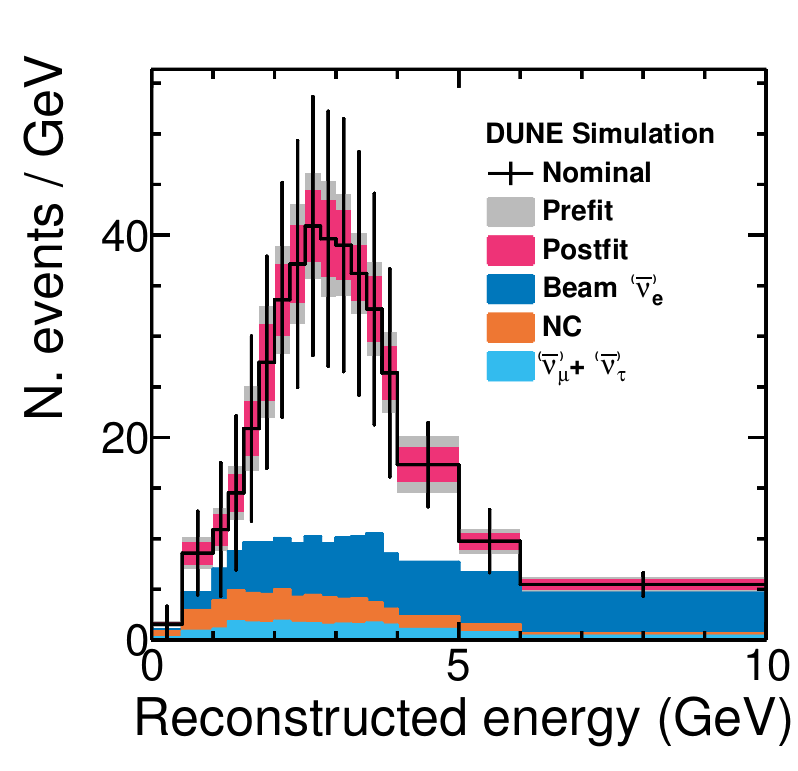
\includegraphics[width=0.8\linewidth]{FD_nue_RHC_ndfd100ktMWyr_allsyst_asimov0_th13_constraint.png}}
 \caption{Reconstructed energy distribution of selected CC $\;\nue^{\bracketbar}$-like events in the FD, for a 50 kt-MW-yr exposure in both FHC and RHC beam modes, for a total 100 kt-MW-yr exposure. The plots are shown for NO, all other oscillation parameters are set to their NuFIT 4.0 best-fit values (see Table~\ref{tab:oscpar_nufit}). The size of the systematic uncertainty bands from all of the flux, cross-section and FD detector systematics used in the analysis are shown, as well as the postfit uncertainty bands with parameters constrained by ND data. Backgrounds are also shown, the largest contribution comes from intrinsic $\nue^{\bracketbar}$ contamination in the beam, although NC and other flavors, $\numu^{\bracketbar} + \nutau^{\bracketbar}$, also contribute.}
 \label{fig:appspectra}
\end{figure}
The expected FD FHC \nue and RHC \anue samples are shown in Figure~\ref{fig:appspectra} for a 100 kt-MW-yr total FD exposure, split equally between FHC and RHC beam modes. The systematic uncertainty bands with and without the ND constraint applied are shown, as well as the background contributions. There are contributions from both \nue and \anue in both beam modes. The NC, intrinsic beam $\nue^{\bracketbar}$ and wrong flavor contamination is also shown; the largest background comes from the intrinsic $\;\nue^{\bracketbar}$ beam contribution in both modes. After a 50 kt-MW-yr exposure in FHC, the \nue sample statistical uncertainty is close to the systematic uncertainty before the ND constraint, although it is still clearly statistics limited when the ND constraint is applied. The \anue sample is still strongly statistics limited after 50 kt-MW-yr exposure in RHC. The difference is largely due to the difference in the \nue and \anue cross sections. %The $\nue^{\bracketbar}$ samples in both modes are clearly statistics limited until much larger exposures.

\begin{figure}[htbp]
  \subfloat[FHC]{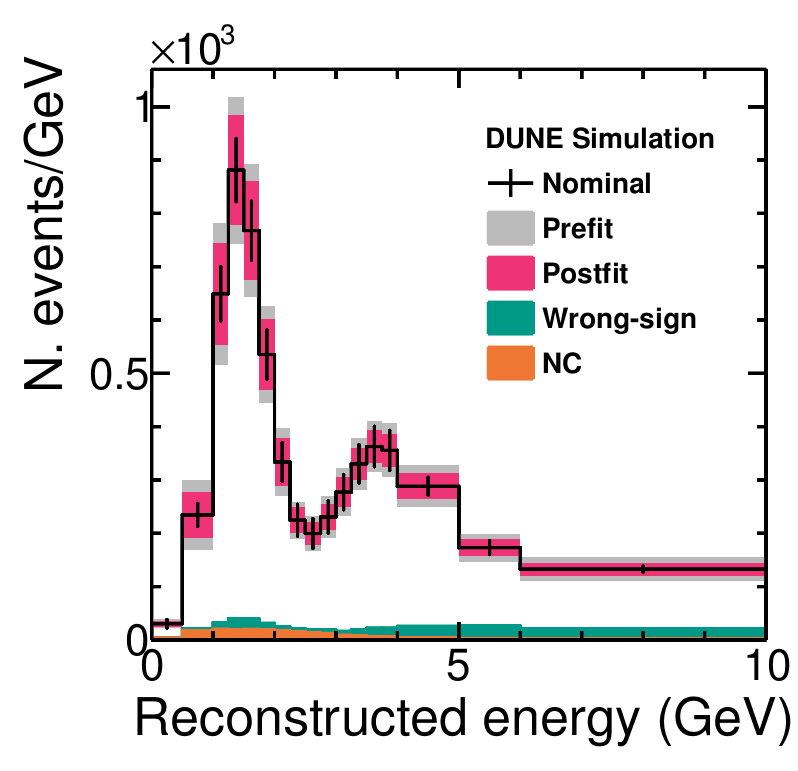
\includegraphics[width=0.8\linewidth]{FD_numu_FHC_ndfd100ktMWyr_allsyst_asimov0_th13_constraint.png}}\\
  \subfloat[RHC]{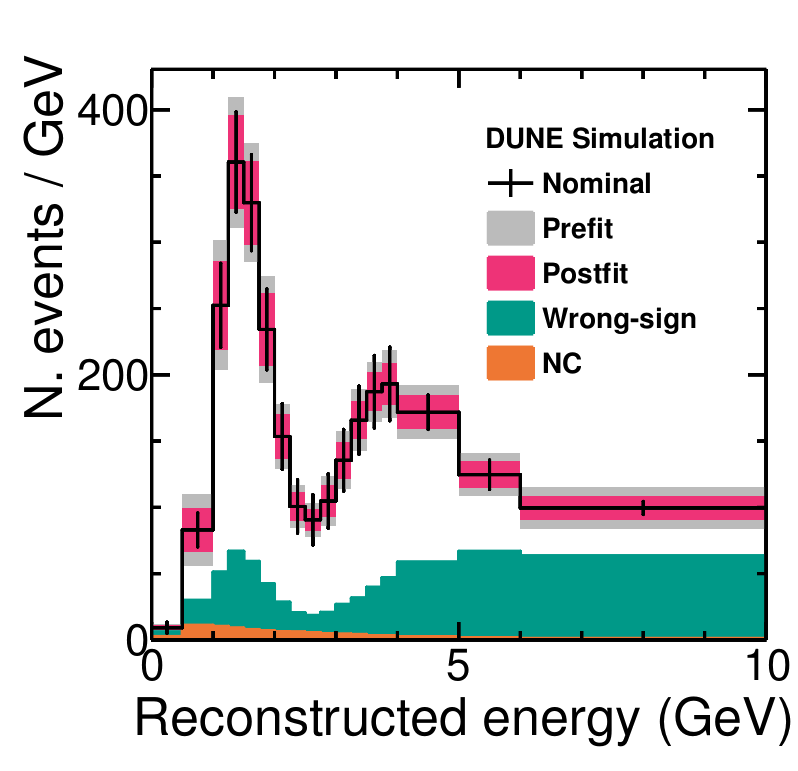
\includegraphics[width=0.8\linewidth]{FD_numu_RHC_ndfd100ktMWyr_allsyst_asimov0_th13_constraint.png}}
\caption{Reconstructed energy distribution of selected CC $\;\nu^{\bracketbar}_{\mu}$-like events in the FD, for 50 kt-MW-yr exposure in both FHC and RHC beam modes, for a total 100 kt-MW-yr exposure. The plots are shown for NO, all other oscillation parameters are set to their NuFIT 4.0 best-fit values (see Table~\ref{tab:oscpar_nufit}). The size of the systematic uncertainty bands from all of the flux, cross-section and ND detector systematics used in the analysis are shown, as well as the postfit uncertainty bands with parameters constrained by ND data. NC backgrounds and wrong-sign contributions to the event rate are also shown.}
\label{fig:disspectra}
\end{figure}
The expected FD FHC \numu and RHC \anumu samples are shown in Figure~\ref{fig:disspectra} for a 100 kt-MW-yr total FD exposure, split equally between FHC and RHC beam modes. The systematic uncertainty bands with and without the ND constraint applied are shown, as well as the background contributions. Although the wrong-sign \numu contribution to the RHC \anumu sample is shown separately, it still provides useful information for constraining the oscillation parameters and is included in the analysis. The statistics are much higher than in Figure~\ref{fig:appspectra}; the statistical uncertainty on the \numu FHC sample is smaller than the systematic uncertainty band for some regions of phase space, even after the ND constraint is applied, although the statistical uncertainty is larger than the constrained systematic uncertainty in the ``dip'' region, around 2.5 GeV, which is likely to have the most impact on the analysis. The statistical uncertainty on the \anumu RHC sample is larger, again due to the smaller \anumu (than \numu) cross section and lower fluxes in RHC running. The statistical uncertainty around the 2.5 GeV dip region is significantly larger than the systematic uncertainty band, although as for the FHC \numu sample, the statistical uncertainty is smaller than the systematics for some regions of the parameter space.

Events with a reconstructed neutrino energy of less than 0.5 GeV (which are shown in Figures~\ref{fig:nd_samples}, ~\ref{fig:appspectra} and~\ref{fig:disspectra}) or a reconstructed neutrino energy greater than 10 GeV are not included in the analysis for any of the FD or ND samples.



